\begin{document}
\begin{flushleft}
 \doublespacing   
    \subsection{How to import project from GitHub}
    1. Open project from GitHub\\
    2. Open "Code" dropdown menu and click "Download ZIP"\\
    \vspace{5mm}
    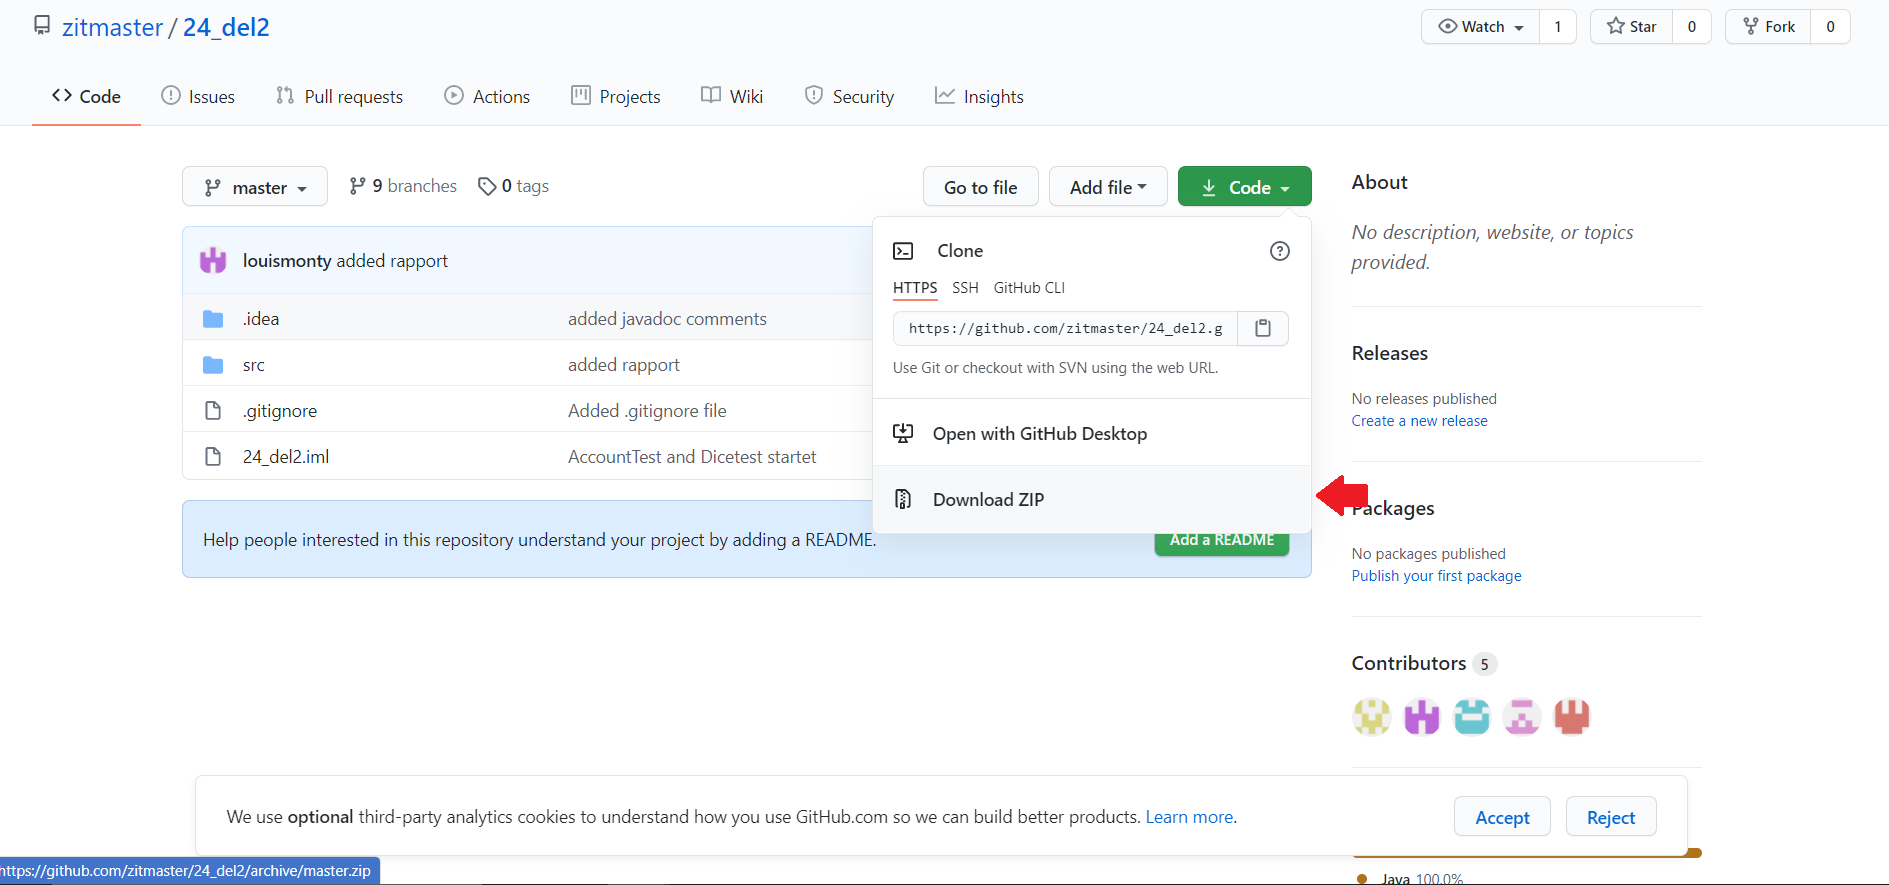
\includegraphics[width=16.5cm]{Report/root/step1.png}\\
    3. Unzip/extract downloaded .zip file to an arbitrary folder\\
    \newpage
    4. Copy the path from unzipped/extracted folder\\
    \begin{verbatim}
    Example: C:\Users\Simon\Dokumenter\Forprojects\24_del2-master\    
    \end{verbatim}
    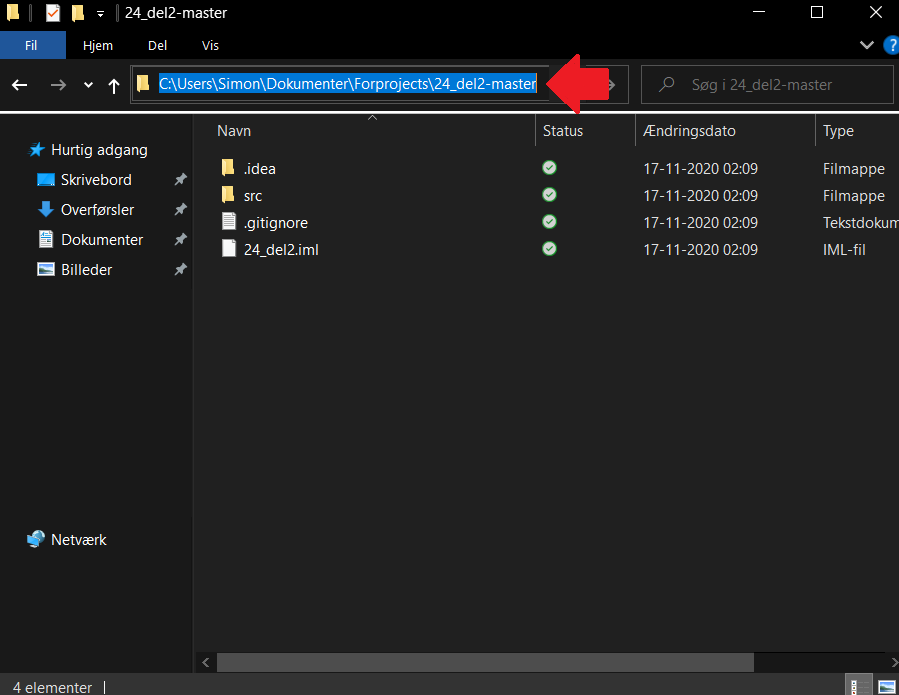
\includegraphics[width=16.5cm]{Report/root/step2.png}\\
    5. Open IntelliJ\\
    \newpage
    6. Click open or Import (if welcome page not shown, skip this step)\\
    \vspace{5mm}
    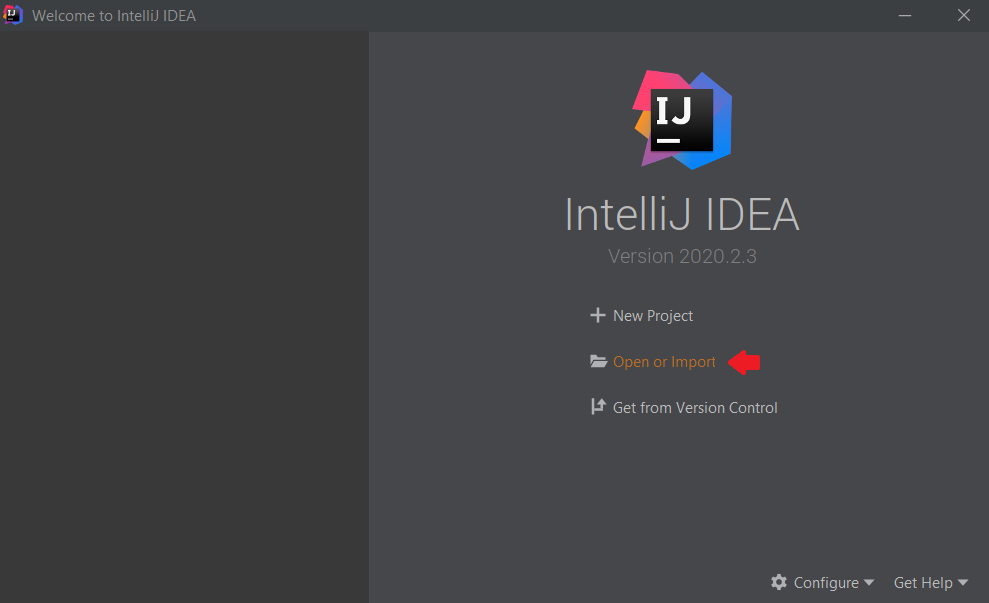
\includegraphics[width=16.5cm]{Report/root/step3.1.png}\\
    7. Click "File" then "Open" (If welcome page was shown, skip this step)\\
    \vspace{5mm}
    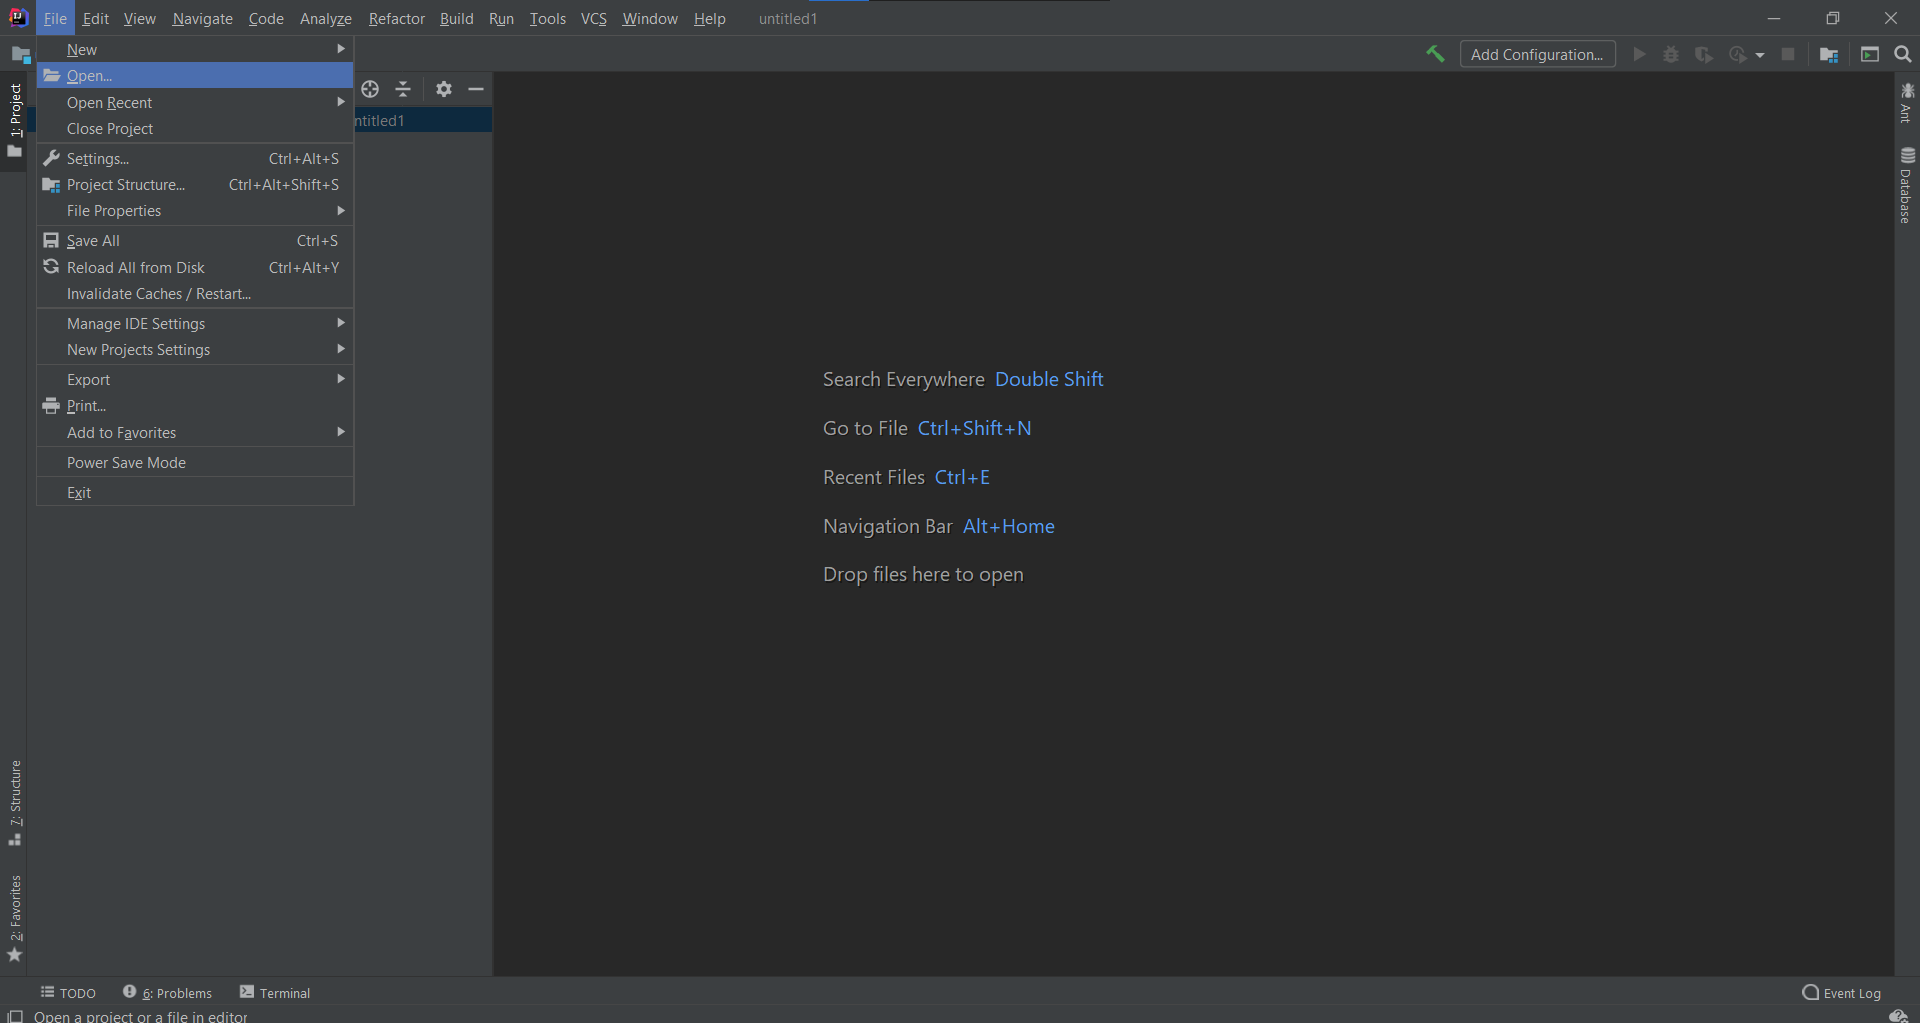
\includegraphics[width=16.5cm]{Report/root/step3.2.png}\\
    \newpage
    8. Paste the copied path and hit enter\\
    \vspace{5mm}
    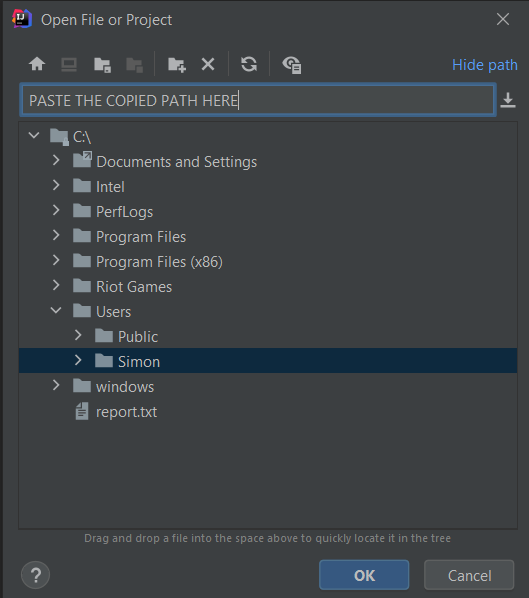
\includegraphics[width=16.5cm]{Report/root/step4.png}\\
    Now the project should be shown and ready to run\\
    \newpage
    It should look like this\\
    \vspace{5mm}
    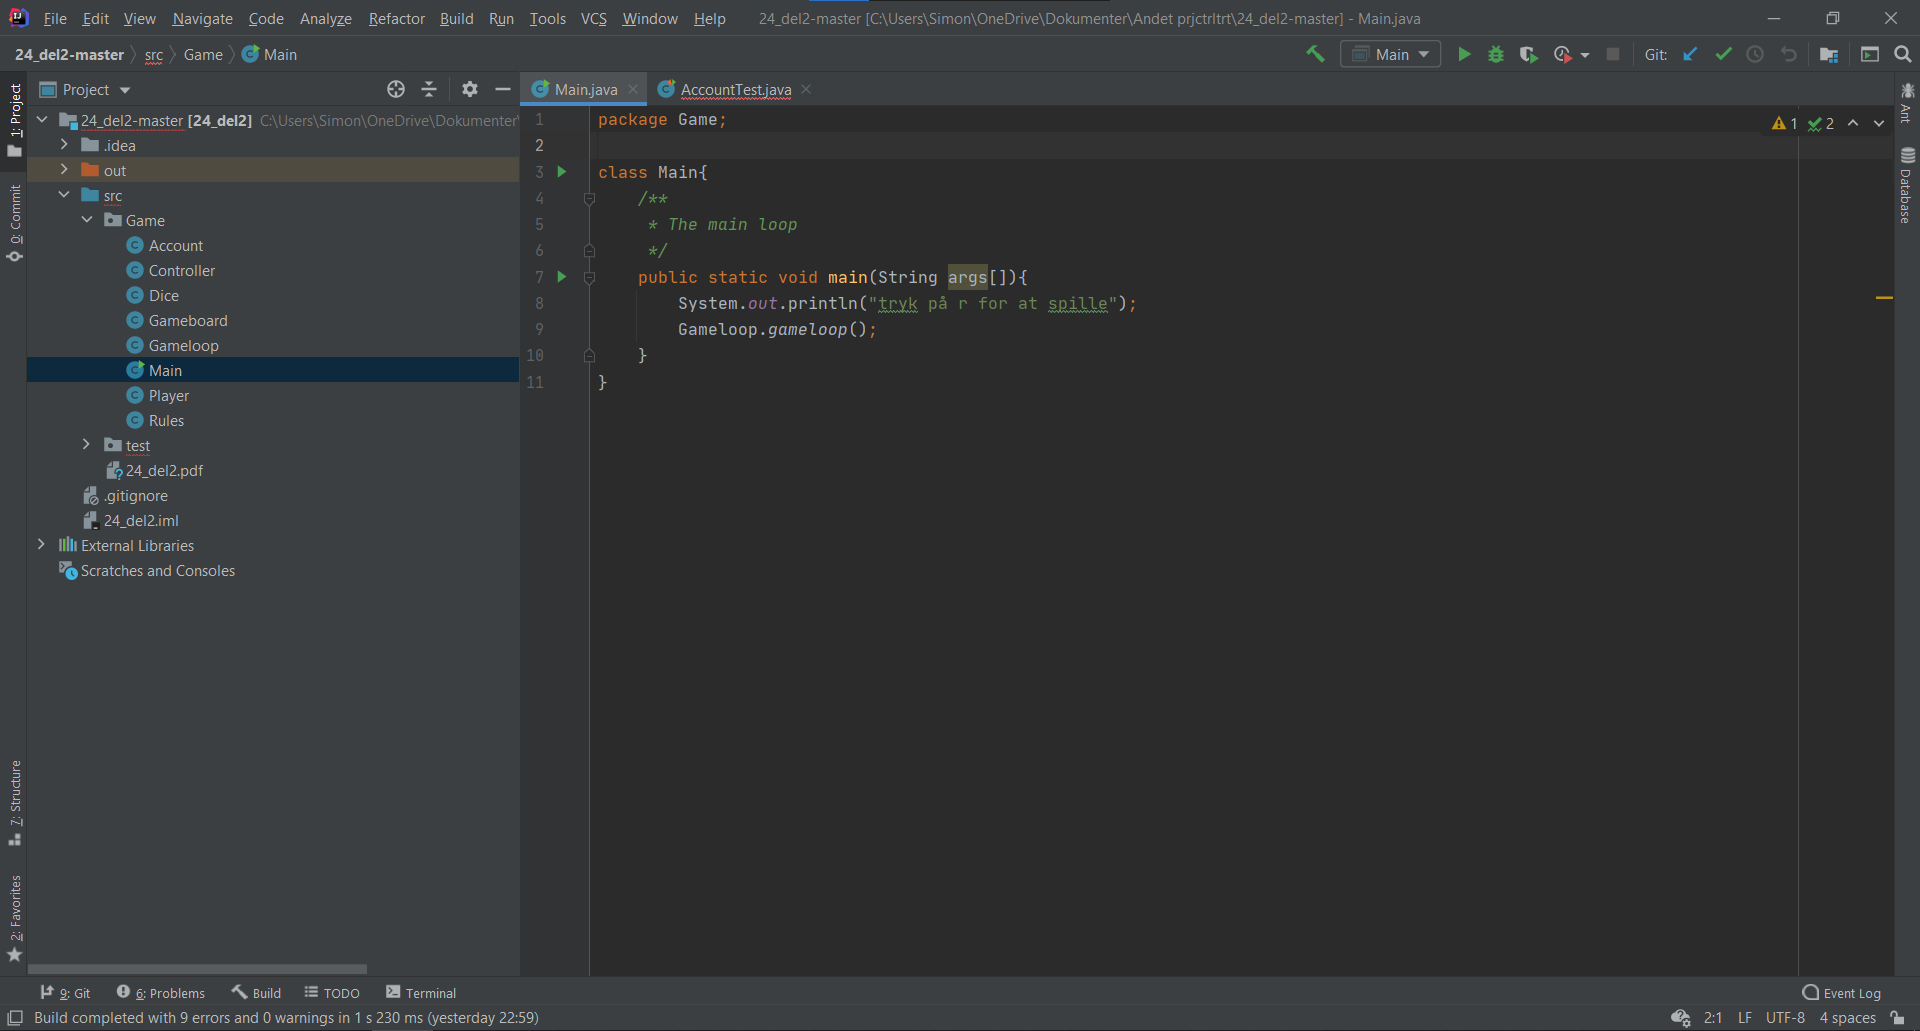
\includegraphics[width=16.5cm]{Report/root/step5.png}\\
    9. To run/execute the project press "Shift" + "F10"

    
    
\end{flushleft}
\end{document}